\section{Zielsetzung}
\label{sec:Zielsetzung}
Es soll das Relaxationsverhalten des Entladevorgangs eines RC-Kreises untersucht werden.

\section{Theorie}
\label{sec:Theorie}

\subsection{Allgemeine Relaxationsgleichung}
\label{sec:AllgemeineRelaxationsgleichung}

Es handelt sich um Relaxationverhalten, wenn ein System aus einem Ausgangszustand ausgelenkt wird und ohne Oszillation in denselben
Zustand zurückkehrt. Allgemein lässt sich eine Differentialgleichung der Form
\begin{align}
    \label{eqn:dA/dt}
    \frac{\symup{d}A}{\symup{d}t} = c[A(t)-A(\infty)]
\end{align}
für die Änderungsgeschwindigkeit der Größe $A$ aufstellen. Diese lässt sich durch Umformung lösen zu
\begin{align}
    \label{eqn:AllgemeineRelaxationsgleichung}
    A(t)=A(\infty)+[A(t)-A(\infty)]e^{ct}.
\end{align}

\subsection{Entladevorgang eines Kondensators}
\label{sec:EntladekurveeinesKondensators}

Die Spannung $U_C$, die auf einem Kondensator mit der Ladung $Q$ und Kapazität $C$, anliegt bestimmt sich durch
\begin{align*}
    U_C=\frac{Q}{C}.
\end{align*}
Wegen des Widerstands $R$ fließt nach dem Ohm'schen Gesetz ein Strom
\begin{align*}
    I=\frac{U_C}{R},
\end{align*}
der für einen Ladungsausgleich sorgt. Die Ladungsänderung auf dem Kondensator ist durch
\begin{align*}
    \symup{d}Q=-I\symup{d}t
\end{align*}
gegeben. Aus diesen Zusammenhängen erhält man die DGL
\begin{align}
    \label{eqn:dQ/dt}
    \frac{\symup{d}Q}{\symup{d}t}=-\frac{Q(t)}{RC},
\end{align}
die eine hohe Ähnlichkeit zu (\ref{eqn:dA/dt}) aufweist. Da der Grenzwert $Q(\infty)$ nicht erreichbar ist, wird er vernachlässigt und die Lösung
der DGL ist durch
\begin{align}
    \label{eqn:Entladung}
    Q(t)=Q(0)e^{-\frac{t}{RC}}
\end{align}
gegeben.

\subsection{Relaxationsverhalten bei angelegter Wechselspannung}
\label{sec:RelaxationsverhaltenbeiangelegterWechselspannung}

Wechselspannung lässt sich im Allgemeinen durch die Funktion
\begin{align*}
    U(t)=U_0 \cdot cos(\omega t)
\end{align*}
beschreiben. Da sich eine Phasenverschiebung zwischen der eingehenden Spannung des Sinusgenerators und der verzögerten Spannung des Kondensators bildet,
ergibt sich für die ausgehende Spannung
\begin{align*}
    U_{C}(t)=A(\omega)\cdot cos(\omega t +\varphi),
\end{align*}
mit der Kondensatorspannungsamplitude $A$. Weiterhin gilt
\begin{align}
    \label{eqn:I(t)}
    I(t)=\frac{\symup{d}Q}{\symup{d}t}=C\frac{\symup{d}U_C}{\symup{d}t}.
\end{align}
Aus den Kirchhoffschen Gesetzen ergibt sich für den RC-Kreis
\begin{align}
    \label{eqn:Kirchhoff}
    U(t)=U_{R}(t)+U_{C}(t).
\end{align}
Aus Formeln (\ref{eqn:dQ/dt}), (\ref{eqn:I(t)}) und (\ref{eqn:Kirchhoff}) und weiteren Umformungen erhält man
\begin{align}
    \label{eqn:Amplitude}
    A(\omega)=\frac{U_0}{\sqrt{1+\omega^2 R^2 C^2}}.
\end{align}

\subsubsection{Phasenverschiebung}
\label{sec:PhasenverschiebungTheorie}
Die Phasenverschiebung $\varphi$ lässt sich aus dem Abstand der Nullstellen $a$der beiden Wellen 
und der Wellenlänge $b$ in Bogenmaß durch
\begin{align}
    \label{eqn:phi}
    \varphi = \frac{a}{b} \cdot 2\pi
\end{align}
ausdrücken.
\begin{figure}
    \centering
    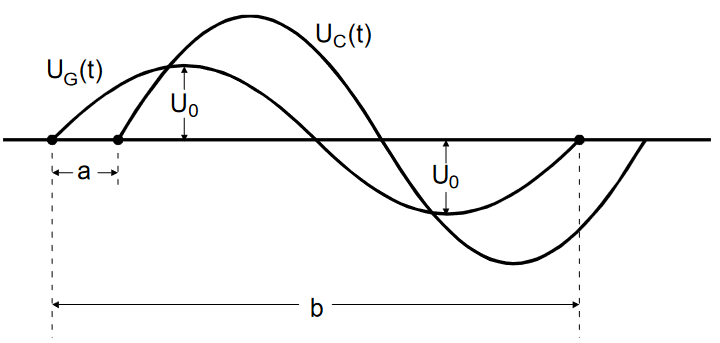
\includegraphics[width=0.7\textwidth]{Phasenverschiebung.png}
    \caption{Skizze zur Phasenverschiebung \cite{sample}.}
    \label{fig:Phasenverschiebung}
\end{figure}

\subsection{Integrationsverhalten eines RC-Kreises}
\label{sec:IntegrationsverhalteneinesRC-Kreises}

Damit ein RC-Kreis als Integrator funktionieren kann, muss $\omega >> \frac{1}{RC}$ gelten.
Gleichung (\ref{eqn:Kirchhoff}) lässt sich umschreiben zu
\begin{align*}
    U(t)&=R \cdot I(t)+U_{C}(t)\\
        &=RC\cdot \frac{\symup{d}U_{C}(t)}{dt}+U_{C}(t).
\end{align*}
Unter der Bedingung $\omega >>\frac{1}{RC}$ löst sich die Gleichung zu
\begin{align}
    \label{eqn:Kondensatorspannung}
    U_{C}(t)=\frac{1}{RC}\int_{0}^{t} U(t')\symup{d}t'.
\end{align}